%% This file was auto-generated by IPython.
%% Conversion from the original notebook file:
%% stat_wells.ipynb
%%
\documentclass[11pt,english,fleqn]{article}

%% This is the automatic preamble used by IPython.  Note that it does *not*
%% include a documentclass declaration, that is added at runtime to the overall
%% document.

\usepackage{amsmath}
\usepackage{amssymb}
\usepackage{graphicx}
\usepackage{ucs}
\usepackage[utf8x]{inputenc}

% needed for markdown enumerations to work
\usepackage{enumerate}

% Slightly bigger margins than the latex defaults
\usepackage{geometry}
\geometry{verbose,tmargin=3cm,bmargin=3cm,lmargin=2.5cm,rmargin=2.5cm}

% Define a few colors for use in code, links and cell shading
\usepackage{color}
\definecolor{orange}{cmyk}{0,0.4,0.8,0.2}
\definecolor{darkorange}{rgb}{.71,0.21,0.01}
\definecolor{darkgreen}{rgb}{.12,.54,.11}
\definecolor{myteal}{rgb}{.26, .44, .56}
\definecolor{gray}{gray}{0.45}
\definecolor{lightgray}{gray}{.95}
\definecolor{mediumgray}{gray}{.8}
\definecolor{inputbackground}{rgb}{.95, .95, .85}
\definecolor{outputbackground}{rgb}{.95, .95, .95}
\definecolor{traceback}{rgb}{1, .95, .95}

% Framed environments for code cells (inputs, outputs, errors, ...).  The
% various uses of \unskip (or not) at the end were fine-tuned by hand, so don't
% randomly change them unless you're sure of the effect it will have.
\usepackage{framed}

% remove extraneous vertical space in boxes
\setlength\fboxsep{0pt}

% codecell is the whole input+output set of blocks that a Code cell can
% generate.

% TODO: unfortunately, it seems that using a framed codecell environment breaks
% the ability of the frames inside of it to be broken across pages.  This
% causes at least the problem of having lots of empty space at the bottom of
% pages as new frames are moved to the next page, and if a single frame is too
% long to fit on a page, will completely stop latex from compiling the
% document.  So unless we figure out a solution to this, we'll have to instead
% leave the codecell env. as empty.  I'm keeping the original codecell
% definition here (a thin vertical bar) for reference, in case we find a
% solution to the page break issue.

%% \newenvironment{codecell}{%
%%     \def\FrameCommand{\color{mediumgray} \vrule width 1pt \hspace{5pt}}%
%%    \MakeFramed{\vspace{-0.5em}}}
%%  {\unskip\endMakeFramed}

% For now, make this a no-op...
\newenvironment{codecell}{}

 \newenvironment{codeinput}{%
   \def\FrameCommand{\colorbox{inputbackground}}%
   \MakeFramed{\advance\hsize-\width \FrameRestore}}
 {\unskip\endMakeFramed}

\newenvironment{codeoutput}{%
   \def\FrameCommand{\colorbox{outputbackground}}%
   \vspace{-1.4em}
   \MakeFramed{\advance\hsize-\width \FrameRestore}}
 {\unskip\medskip\endMakeFramed}

\newenvironment{traceback}{%
   \def\FrameCommand{\colorbox{traceback}}%
   \MakeFramed{\advance\hsize-\width \FrameRestore}}
 {\endMakeFramed}

% Use and configure listings package for nicely formatted code
\usepackage{listingsutf8}
\lstset{
  language=python,
  inputencoding=utf8x,
  extendedchars=\true,
  aboveskip=\smallskipamount,
  belowskip=\smallskipamount,
  xleftmargin=2mm,
  breaklines=true,
  basicstyle=\small \ttfamily,
  showstringspaces=false,
  keywordstyle=\color{blue}\bfseries,
  commentstyle=\color{myteal},
  stringstyle=\color{darkgreen},
  identifierstyle=\color{darkorange},
  columns=fullflexible,  % tighter character kerning, like verb
}

% The hyperref package gives us a pdf with properly built
% internal navigation ('pdf bookmarks' for the table of contents,
% internal cross-reference links, web links for URLs, etc.)
\usepackage{hyperref}
\hypersetup{
  breaklinks=true,  % so long urls are correctly broken across lines
  colorlinks=true,
  urlcolor=blue,
  linkcolor=darkorange,
  citecolor=darkgreen,
  }

% hardcode size of all verbatim environments to be a bit smaller
\makeatletter 
\g@addto@macro\@verbatim\small\topsep=0.5em\partopsep=0pt
\makeatother 

% Prevent overflowing lines due to urls and other hard-to-break entities.
\sloppy

\setlength{\mathindent}{0pt}
\setlength{\parindent}{0pt}
\setlength{\parskip}{8pt}
\begin{document}

\begin{codecell}
\begin{codeinput}
\begin{lstlisting}
from pandas import *
from statsmodels.formula.api import logit
from statsmodels.nonparametric import KDE
from patsy import dmatrix, dmatrices
\end{lstlisting}
\end{codeinput}
\end{codecell}
\section{Banglades'te su kuyusu degisiminin lojistik modeli}

Bu analiz Gelman ve Hill'in kitabi \emph{Data Analysis Using Regression
and Multilevel/Hierarchical Models} 5.4'uncu bolumu isliyor.

Verimizde 3,000 haneye gidilerek anketle toplanmis veri var. Veride
hanelerin yakinlarindaki kuyudaki arsenik seviyesi toplanmis, ve
paylasilan verideki tum hanelerin kuyular sagliksiz seviyede arsenik
iceriyor. Verideki diger bilgiler en yakindaki ``saglikli'' bir kuyuya
yakinlik, ve o hanenin bu saglikli su kuyusuna (bir sene sonra yapilan
kontrole gore) gecip gecmedigi. Ayrica hanede fikri sorulan kisinin
egitim seviyesi ve bu hanedeki kisilerin herhangi bir sosyal topluluga
(community assocation) ait olup olmadiklari.

Amacimiz su kuyusunun degisimini modellemek. Bu eylem olup / olmama
baglaminda evet / hayir seklinde bir degisken oldugu icin ikili (binary)
olarak temsil edilebilir ve ikili cevaplar / sonuclar lojistik regresyon
ile modellenebilirler.

Veriye bakalim.

\begin{codecell}
\begin{codeinput}
\begin{lstlisting}
df = read_csv('wells.dat', sep = ' ', header = 0, index_col = 0)
print df.head()
\end{lstlisting}
\end{codeinput}
\begin{codeoutput}
\begin{verbatim}
switch  arsenic       dist  assoc  educ
1       1     2.36  16.826000      0     0
2       1     0.71  47.321999      0     0
3       0     2.07  20.966999      0    10
4       1     1.15  21.486000      0    12
5       1     1.10  40.874001      1    14
\end{verbatim}
\end{codeoutput}
\end{codecell}
\subsection{Model 1: Guvenli su kuyusuna uzaklik}

Ilk once modelde kuyu uzakligini kullanalim.

\begin{codecell}
\begin{codeinput}
\begin{lstlisting}
model1 = logit('switch ~ dist', df = df).fit()
print model1.summary()

\end{lstlisting}
\end{codeinput}
\begin{codeoutput}
\begin{verbatim}
Optimization terminated successfully.
         Current function value: 2038.118913
         Iterations 4
                           Logit Regression Results                           
==============================================================================
Dep. Variable:                 switch   No. Observations:                 3020
Model:                          Logit   Df Residuals:                     3018
Method:                           MLE   Df Model:                            1
Date:                Sat, 16 Feb 2013   Pseudo R-squ.:                 0.01017
Time:                        12:46:35   Log-Likelihood:                -2038.1
converged:                       True   LL-Null:                       -2059.0
                                        LLR p-value:                 9.798e-11
==============================================================================
                 coef    std err          z      P>|z|      [95.0% Conf. Int.]
------------------------------------------------------------------------------
Intercept      0.6060      0.060     10.047      0.000         0.488     0.724
dist          -0.0062      0.001     -6.383      0.000        -0.008    -0.004
==============================================================================
\end{verbatim}
\end{codeoutput}
\end{codecell}
Uzaklik (dist) icin elde edilen katsayi -0.0062, fakat bu sayi kafa
karistirici olabilir cunku uzaklik metre olarak olculur, o zaman bu
katsayi mesela 90 metre ile 91 metre uzakligin degisime olan etkisini
olcmektedir, kisacasi pek faydali degildir. Yani uzaklik metre ile
olculdugu icin 1 metrenin modeldeki etkisi ufak, o yuzden bu olcutu
olceklersek (scale) belki regresyon katsayilarimiz daha net cikar.

Bunu nasil yapacagiz? Olceklenmis yeni bir degisken yaratmak yerine, onu
formulun icinde tanimlayabiliriz. Burada bir ara not: eger formul icinde
+,- gibi operasyonlari aritmetik islem olarak kullanmak istiyorsak, o
zaman `I()' cagrisini yapmak lazim, cunku + operasyonu mesela Patsy
formullerinde baska amaclar icin kullaniliyor. `I' harfi birim
(identity) kelimesinden geliyor, yani hicbir seyin degismedigini
anlatmaya ugrasiyoruz, ``icinde ne varsa onu ver'' diyoruz {[}1{]}.

\begin{codecell}
\begin{codeinput}
\begin{lstlisting}
model1 = logit('switch ~I(dist/100.)', df = df).fit()
print model1.summary()
\end{lstlisting}
\end{codeinput}
\begin{codeoutput}
\begin{verbatim}
Optimization terminated successfully.
         Current function value: 2038.118913
         Iterations 4
                           Logit Regression Results                           
==============================================================================
Dep. Variable:                 switch   No. Observations:                 3020
Model:                          Logit   Df Residuals:                     3018
Method:                           MLE   Df Model:                            1
Date:                Sat, 16 Feb 2013   Pseudo R-squ.:                 0.01017
Time:                        13:02:29   Log-Likelihood:                -2038.1
converged:                       True   LL-Null:                       -2059.0
                                        LLR p-value:                 9.798e-11
==================================================================================
                     coef    std err          z      P>|z|      [95.0% Conf. Int.]
----------------------------------------------------------------------------------
Intercept          0.6060      0.060     10.047      0.000         0.488     0.724
I(dist / 100.)    -0.6219      0.097     -6.383      0.000        -0.813    -0.431
==================================================================================
\end{verbatim}
\end{codeoutput}
\end{codecell}
Simdi modelimizi grafikleyelim. Yanliz degisim (switch) verisini suni
olarak kaydirmamiz / segirtmemiz (jitter) gerekiyor, cunku degisim 0 ve
1'den baska bir sey olamaz ve grafik surekli ayni iki bolgeye nokta
basip duracak.

\begin{codecell}
\begin{codeinput}
\begin{lstlisting}
def binary_jitter(x, jitter_amount = .05):
    '''
    0/1 vektoru iceren veriye segirtme ekle
    '''
    jitters = np.random.rand(*x.shape) * jitter_amount
    x_jittered = x + np.where(x == 1, -1, 1) * jitters
    return x_jittered
\end{lstlisting}
\end{codeinput}
\end{codecell}
\begin{codecell}
\begin{codeinput}
\begin{lstlisting}
plt.plot(df['dist'], binary_jitter(df['switch'], .1), '.', alpha = .1)
plt.plot(np.sort(df['dist']), model1.predict()[np.argsort(df['dist'])], lw = 2)
plt.ylabel('Switched Wells')
plt.xlabel('Distance from safe well (meters)')
\end{lstlisting}
\end{codeinput}
\begin{codeoutput}
\begin{verbatim}
<matplotlib.text.Text at 0xa435acc>
\end{verbatim}
\begin{center}
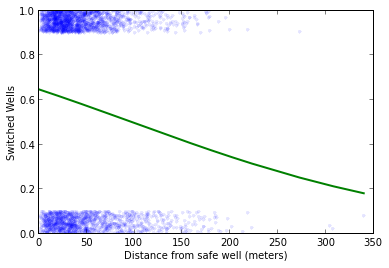
\includegraphics[width=0.7\textwidth]{stat_wells_files/stat_wells_fig_00.png}
\par
\end{center}
\end{codeoutput}
\end{codecell}
Mavi noktalar gercek veri, yesil cizgi ise uzaklik gecilerek modelin
olusturdugu ``tahmin''. Modelin gercek veriye ne kadar uydugunu
goruyoruz boylece, yesil cizginin yuksek olasilik verdigi bolgelerde ust
kismin daha mavi olmasini bekleriz mesela. Ustteki resimde asagi yukari
bunu gosteriyor.

Bir problemin grafiklemesine baska bir yonden yaklasalim, kuyu
degistirenlerin degisim uzakliginin yogunlugu, bir de kuyu
degistirmeyenlerin degisim uzakliginin yogunlugu. Degisimi yapanlarin
dagilimina bakinca, kisa mesafelerde daha fazla yogunluk gormeyi
bekliyoruz, degistirmeyenlerin ise uzun mesafelerde daha fazla yogunlugu
olur herhalde.

Yogunlugu gostermek icin cekirdek yogunluk hesabi (kernel density
estimation) teknigini kullaniyoruz. Bu teknik her veri noktasina
Gaussian, kutu (box), ya da diger turden bir ``cekirdek'' fonksiyonunu
koyar (ve veriyi o fonksiyona gecer, sonucu kaydeder), ve bu is bitince
tum cekirdekler ust uste toplanarak genel dagilim ortaya cikartilir.
Teknik histogram teknigiyle ayni isi yapmaya ugrasir, bir anlamda
verinin dagilimini daha puruzsuz (smooth) hale getirir.

Bu teknik istatistikte oldukca yeni bir teknik sayilir, kullanilmasi
icin bilgisayar hesabi gerekiyor (kiyasla histogram elle de
yapilabilir), yeni hesapsal tekniklerde olan ilerlemelerin veri
analizine getirdigi bir yenilik yani!

\begin{codecell}
\begin{codeinput}
\begin{lstlisting}
kde_sw = KDE(df['dist'][df['switch'] == 1])
kde_nosw = KDE(df['dist'][df['switch'] == 0])

kde_sw.fit()
kde_nosw.fit()

plt.plot(kde_sw.support, kde_sw.density, label = 'Switch')
plt.plot(kde_nosw.support, kde_nosw.density, color = 'red', label = 'No Switch')
plt.xlabel('Distance (meters)')
plt.legend(loc = 'best')
\end{lstlisting}
\end{codeinput}
\begin{codeoutput}
\begin{verbatim}
<matplotlib.legend.Legend at 0x109da8b50>
\end{verbatim}
\begin{center}
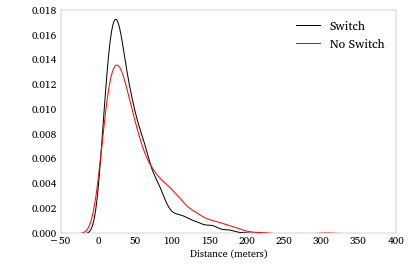
\includegraphics[width=0.7\textwidth]{stat_wells_files/stat_wells_fig_01.png}
\par
\end{center}
\end{codeoutput}
\end{codecell}
\subsection{Model 2: Guvenli kuyuya olan uzaklik ve kendi kuyusunun
arsenik seviyesi}

Simdi arsenik seviyesini modelimize ekleyelim. Bekleriz ki kuyusunda
yuksek arsenik miktari olan kimselerin kuyu degistirmesi daha cok
beklenen bir seydir.

\begin{codecell}
\begin{codeinput}
\begin{lstlisting}
model2 = logit('switch ~ I(dist / 100.) + arsenic', df = df).fit()
print model2.summary()
\end{lstlisting}
\end{codeinput}
\begin{codeoutput}
\begin{verbatim}
Optimization terminated successfully.
         Current function value: 1965.334134
         Iterations 5
                           Logit Regression Results                           
==============================================================================
Dep. Variable:                 switch   No. Observations:                 3020
Model:                          Logit   Df Residuals:                     3017
Method:                           MLE   Df Model:                            2
Date:                Sat, 22 Dec 2012   Pseudo R-squ.:                 0.04551
Time:                        13:05:29   Log-Likelihood:                -1965.3
converged:                       True   LL-Null:                       -2059.0
                                        LLR p-value:                 1.995e-41
==================================================================================
                     coef    std err          z      P>|z|      [95.0% Conf. Int.]
----------------------------------------------------------------------------------
Intercept          0.0027      0.079      0.035      0.972        -0.153     0.158
I(dist / 100.)    -0.8966      0.104     -8.593      0.000        -1.101    -0.692
arsenic            0.4608      0.041     11.134      0.000         0.380     0.542
==================================================================================
\end{verbatim}
\end{codeoutput}
\end{codecell}
Ki katsayilar da aynen bunu gosteriyor. Guvenli kuyuya olan uzaklik
buyudukce degisime negatif etki yapiyor ama kendi kuyusundaki arsenik
seviyesinin artmasi degisimde pozitif etki yapiyor.

\subsubsection{Bilesen (marginal) etkiler}

Tum bu degiskenlerin degisim olasiligi uzerindeki etkilerini gormek icin
verinin ortalama noktasinda bir bilesen hesabi yapalim.

\begin{codecell}
\begin{codeinput}
\begin{lstlisting}
model2.margeff(at = 'mean')
\end{lstlisting}
\end{codeinput}
\begin{codeoutput}
\begin{verbatim}
array([-0.21806505,  0.11206108])
\end{verbatim}
\end{codeoutput}
\end{codecell}
Bu sonuca gore, ankette soru sorulan ortalama kisi icin en yakin kuyuya
olan uzaklikta 100 metrelik bir degisim olasiliginda \%22 dusus anlamina
gelmektedir. Fakat kendi kuyusundaki arsenikte 1 seviyesinde bir artis
degisim olasiligini \%11 oraninda arttirmaktadir.

\subsubsection{Siniflarin ayirilabilirligi}

Bu modelin kuyu degistirenler ile degistirmeyenleri ne kadar iyi
siniflayabildigini anlamak icin her siniftaki kisiyi uzaklik-arsenik
uzayinda grafikleyebiliriz.

Biz pek bir iyi bir ayirim goremedik, o sebeple modelin oldukca yuksek
bir hata oraninin olmasini bekliyoruz. Fakat baska bir sey farkediyoruz,
grafigin ``kisa mesafe-yuksek arsenik'' bolgesinde cogunlukla
degisimciler var, ve ``uzun mesafe-dusuk arsenik'' bolgesinde cogunlukla
degistirmeyenler var.

\begin{codecell}
\begin{codeinput}
\begin{lstlisting}
logit_pars = model2.params
intercept = -logit_pars[0] / logit_pars[2]
slope = -logit_pars[1] / logit_pars[2]

dist_sw = df['dist'][df['switch'] == 1]
dist_nosw = df['dist'][df['switch'] == 0]
arsenic_sw = df['arsenic'][df['switch'] == 1]
arsenic_nosw = df['arsenic'][df['switch'] == 0]
plt.figure(figsize = (12, 8))
plt.plot(dist_sw, arsenic_sw, '.', mec = 'purple', mfc = 'None', 
         label = 'Switch')
plt.plot(dist_nosw, arsenic_nosw, '.', mec = 'orange', mfc = 'None', 
         label = 'No switch')
plt.plot(np.arange(0, 350, 1), intercept + slope * np.arange(0, 350, 1) / 100.,
         '-k', label = 'Separating line')
plt.ylim(0, 10)
plt.xlabel('Distance to safe well (meters)')
plt.ylabel('Arsenic level')
plt.legend(loc = 'best')
\end{lstlisting}
\end{codeinput}
\begin{codeoutput}
\begin{verbatim}
<matplotlib.legend.Legend at 0x109f7cb10>
\end{verbatim}
\begin{center}
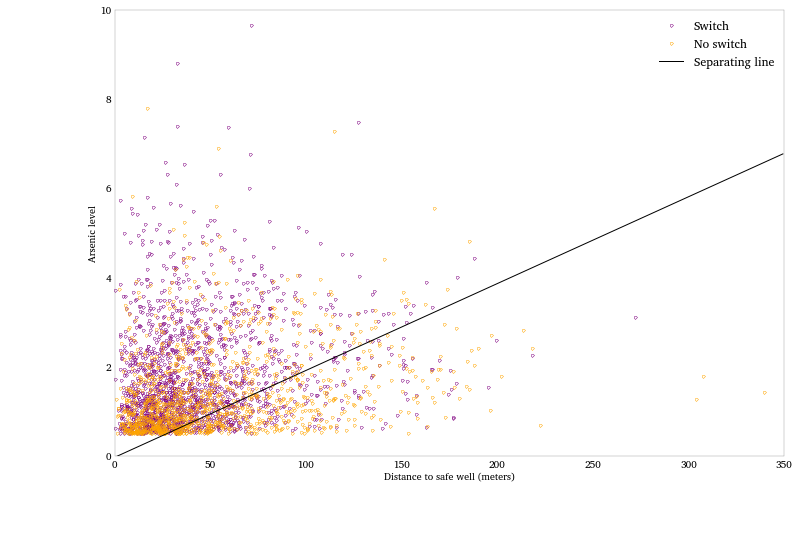
\includegraphics[width=0.7\textwidth]{stat_wells_files/stat_wells_fig_02.png}
\par
\end{center}
\end{codeoutput}
\end{codecell}
\subsection{Model 3: Etkilesim eklemek}

Arsenik seviyesi ve uzaklik degiskenlerinin modele ayri ayri yaptigi
etkiler yaninda, beraber olarak ta bazi etkiler yapacagini
dusunebiliriz. 100 metrelik mesafenin degisim kararina olan etkisi
kuyunuzdaki arsenik seviyesiyle baglantili olabilmesi.. Insanlarin boyle
dusunmesini bekleyebiliriz, yani, bu problem baglaminda, tipik kisi
durup ta ``once arsenik yokmus gibi dusuneyim, sadece mesafeye
bakayim'', sonra ``simdi arsenigi dusuneyim, mesafe yokmus gibi
yapayim'', ve bunlardan sonra ``simdi bu iki ayri karari ust uste
koyayim'' seklinde dusunmez.

Patsy ile modele etkilesim eklemenin yolu degiskenler arasinda
\texttt{:} operatorunu kullanmak ile olur.

\begin{codecell}
\begin{codeinput}
\begin{lstlisting}
model3 = logit('switch ~ I(dist / 100.) + arsenic + I(dist / 100.):arsenic', 
                   df = df).fit()
print model3.summary()
\end{lstlisting}
\end{codeinput}
\begin{codeoutput}
\begin{verbatim}
Optimization terminated successfully.
         Current function value: 1963.814202
         Iterations 5
                           Logit Regression Results                           
==============================================================================
Dep. Variable:                 switch   No. Observations:                 3020
Model:                          Logit   Df Residuals:                     3016
Method:                           MLE   Df Model:                            3
Date:                Sat, 22 Dec 2012   Pseudo R-squ.:                 0.04625
Time:                        13:05:33   Log-Likelihood:                -1963.8
converged:                       True   LL-Null:                       -2059.0
                                        LLR p-value:                 4.830e-41
==========================================================================================
                             coef    std err          z      P>|z|      [95.0% Conf. Int.]
------------------------------------------------------------------------------------------
Intercept                 -0.1479      0.118     -1.258      0.208        -0.378     0.083
I(dist / 100.)            -0.5772      0.209     -2.759      0.006        -0.987    -0.167
arsenic                    0.5560      0.069      8.021      0.000         0.420     0.692
I(dist / 100.):arsenic    -0.1789      0.102     -1.748      0.080        -0.379     0.022
==========================================================================================
\end{verbatim}
\end{codeoutput}
\end{codecell}
Sonuca gore etkilesimin katsayisi negatif ve istatistiki olarak anlamli
(significant) {[}3{]}. Bu katsayinin degisim uzerindeki etkisini nicesel
olarak hemen bakar bakmaz anlayamiyor olsak bile, niteliksel olarak
etkisi sezgilerimiz ile uyusuyor. Uzaklik degisimde negatif etkili, ama
bu negatif etki yuksek arsenik seviyesi devreye girince azaliyor. Diger
yandan arsenik seviyesinin degisimde pozitif etkisi var, ama o etki en
yakin kuyu mesafesi arttikca azaliyor.

\subsection{Model 4: Egitim seviyesi ve ek bazi etkilesimler, ve
degiskenleri ortalamak}

Egitim seviyesi kisilerin arsenigin kotu etkilerini anlamasinda pozitif
etki yapmasi beklenir, ve bu sebeple egitim seviyesi degisim kararina
pozitif etki yapmalidir. Elimizdeki veride egitim yil bazinda
kayitlanmis, biz bu veri noktasini olcekleyecegiz (aynen uzakliga
yaptimiz gibi, cunku egitimde 1 senelik degisimin pek bir anlami yok),
bunu icin 4'e bolecegiz. Ayrica bu yeni degiskenin diger degiskenler ile
etkilesimini devreye sokacagiz.

Ek olarak tum degiskenleri ortalayacagiz ki boylece onlari yorumlamamiz
rahatlasacak. Bir kez daha bu isi tamamen Patsy sayesinde formul icinde
halledecegiz, disaridan on hesap yapip formule gecmemiz gerekmeyecek.

\begin{codecell}
\begin{codeinput}
\begin{lstlisting}
model_form = ('switch ~ center(I(dist / 100.)) + center(arsenic) + ' +
              'center(I(educ / 4.)) + ' +
              'center(I(dist / 100.)) : center(arsenic) + ' + 
              'center(I(dist / 100.)) : center(I(educ / 4.)) + ' + 
              'center(arsenic) : center(I(educ / 4.))'
             )
model4 = logit(model_form, df = df).fit()
print model4.summary()
\end{lstlisting}
\end{codeinput}
\begin{codeoutput}
\begin{verbatim}
Optimization terminated successfully.
         Current function value: 1945.871775
         Iterations 5
                           Logit Regression Results                           
==============================================================================
Dep. Variable:                 switch   No. Observations:                 3020
Model:                          Logit   Df Residuals:                     3013
Method:                           MLE   Df Model:                            6
Date:                Sat, 22 Dec 2012   Pseudo R-squ.:                 0.05497
Time:                        13:05:35   Log-Likelihood:                -1945.9
converged:                       True   LL-Null:                       -2059.0
                                        LLR p-value:                 4.588e-46
===============================================================================================================
                                                  coef    std err          z      P>|z|      [95.0% Conf. Int.]
---------------------------------------------------------------------------------------------------------------
Intercept                                       0.3563      0.040      8.844      0.000         0.277     0.435
center(I(dist / 100.))                         -0.9029      0.107     -8.414      0.000        -1.113    -0.693
center(arsenic)                                 0.4950      0.043     11.497      0.000         0.411     0.579
center(I(educ / 4.))                            0.1850      0.039      4.720      0.000         0.108     0.262
center(I(dist / 100.)):center(arsenic)         -0.1177      0.104     -1.137      0.256        -0.321     0.085
center(I(dist / 100.)):center(I(educ / 4.))     0.3227      0.107      3.026      0.002         0.114     0.532
center(arsenic):center(I(educ / 4.))            0.0722      0.044      1.647      0.100        -0.014     0.158
===============================================================================================================
\end{verbatim}
\end{codeoutput}
\end{codecell}
\subsubsection{Modelin basarisini irdelemek: Kutulanmis Kalinti
grafikleri (Binned Residual plots)}

Model kalintisinin (yani model ile gercek veri arasindaki hatalar
-residual-) ile ayri ayri her degisken ile grafikleri, uzaklik-kalinti,
arsenik-kalinti gibi, bizi modelde gayri lineerlik olup olmadigi
hakkinda uyarabilir. Cunku kalintinin Gaussian bir dagilimda olmasini
bekleriz, model hatasi tam anlamiyla bir ``gurultu'' halinde olmalidir,
ki dogada gurultunun tanimi Gaussian dagilimina sahip olmaktir. Eger bu
grafikte kabaca her yere esit sekilde dagilmis bir goruntu gormuyorsak,
o zaman modelimizde yakalayamadigimiz bir gayri lineerlik (nonlinearity)
vardir, ya da, birbirinden farkli olan kalinti grafikleri kalintilari
dagilimlarinin birbirinden farkli oldugunun isaretidir
(heteroskedasticity).

Ikili bir modelde kalintilari ham sekilde grafiklemenin pek anlami
yoktur, o sebeple biraz puruzsuzlestirme uygulayacagiz. Altta
degiskenler icin olusturdugumuz kutucuklar (bins) icine kalintilarin
ortalamasini koyacagiz ve bunlari grafikleyecegiz (lowess ya da
hareketli ortalama -moving average- teknigi de burada ise
yarayabilirdi).

\begin{codecell}
\begin{codeinput}
\begin{lstlisting}
def bin_residuals(resid, var, bins):
    '''
    Compute average residuals within bins of a variable.
    
    Returns a dataframe indexed by the bins, with the bin midpoint,
    the residual average within the bin, and the confidence interval 
    bounds.
    '''
    resid_df = DataFrame({'var': var, 'resid': resid})
    resid_df['bins'] = qcut(var, bins)
    bin_group = resid_df.groupby('bins')
    bin_df = bin_group['var', 'resid'].mean()
    bin_df['count'] = bin_group['resid'].count()
    bin_df['lower_ci'] = -2 * (bin_group['resid'].std() / 
                               np.sqrt(bin_group['resid'].count()))
    bin_df['upper_ci'] =  2 * (bin_group['resid'].std() / 
                               np.sqrt(bin_df['count']))
    bin_df = bin_df.sort('var')
    return(bin_df)

def plot_binned_residuals(bin_df):
    '''
    Plotted binned residual averages and confidence intervals.
    '''
    plt.plot(bin_df['var'], bin_df['resid'], '.')
    plt.plot(bin_df['var'], bin_df['lower_ci'], '-r')
    plt.plot(bin_df['var'], bin_df['upper_ci'], '-r')
    plt.axhline(0, color = 'gray', lw = .5)
    
arsenic_resids = bin_residuals(model4.resid, df['arsenic'], 40)
dist_resids = bin_residuals(model4.resid, df['dist'], 40)
plt.figure(figsize = (12, 5))
plt.subplot(121)
plt.ylabel('Residual (bin avg.)')
plt.xlabel('Arsenic (bin avg.)')
plot_binned_residuals(arsenic_resids)
plt.subplot(122)
plot_binned_residuals(dist_resids)
plt.ylabel('Residual (bin avg.)')
plt.xlabel('Distance (bin avg.)')
\end{lstlisting}
\end{codeinput}
\begin{codeoutput}
\begin{verbatim}
<matplotlib.text.Text at 0x10ae3ef50>
\end{verbatim}
\begin{center}
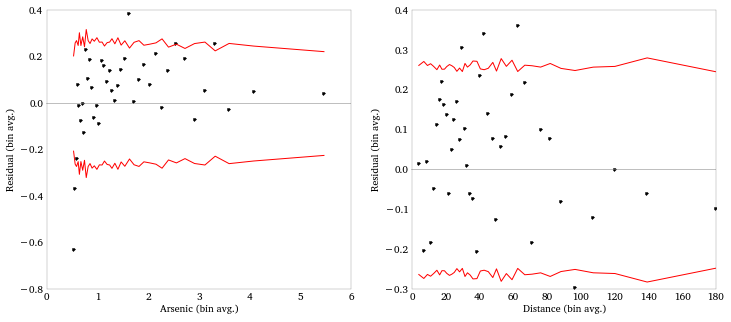
\includegraphics[width=0.7\textwidth]{stat_wells_files/stat_wells_fig_03.png}
\par
\end{center}
\end{codeoutput}
\end{codecell}
\subsection{Model 5: arsenigi log olceklemek}

Kutulanmis artik grafiklerine bakinca arsenik degiskeninde biraz gayri
lineerlik goruyoruz, cunku noktalarin dagilimi cok fazla belli bir
bolgede. Dikkat edelim, model nasil dusuk arsenigi gercekte oldugundan
daha fazla olacagini tahmin etmis (overestimate), ayrica yuksek arsenigi
gercekte oldugundan daha az olacagini tahmin etmis (underestimate). Bu
bize arsenik degiskeni uzerinde belki de log transformasyonu gibi bir
seyler yapmamizin gerektiginin isareti.

Bu degisimi de direk formul icinde yapabiliriz.

\begin{codecell}
\begin{codeinput}
\begin{lstlisting}
model_form = ('switch ~ center(I(dist / 100.)) + center(np.log(arsenic)) + ' +
              'center(I(educ / 4.)) + ' +
              'center(I(dist / 100.)) : center(np.log(arsenic)) + ' + 
              'center(I(dist / 100.)) : center(I(educ / 4.)) + ' + 
              'center(np.log(arsenic)) : center(I(educ / 4.))'
             )

model5 = logit(model_form, df = df).fit()
print model5.summary()
\end{lstlisting}
\end{codeinput}
\begin{codeoutput}
\begin{verbatim}
Optimization terminated successfully.
         Current function value: 1931.554102
         Iterations 5
                           Logit Regression Results                           
==============================================================================
Dep. Variable:                 switch   No. Observations:                 3020
Model:                          Logit   Df Residuals:                     3013
Method:                           MLE   Df Model:                            6
Date:                Sat, 22 Dec 2012   Pseudo R-squ.:                 0.06192
Time:                        13:05:57   Log-Likelihood:                -1931.6
converged:                       True   LL-Null:                       -2059.0
                                        LLR p-value:                 3.517e-52
==================================================================================================================
                                                     coef    std err          z      P>|z|      [95.0% Conf. Int.]
------------------------------------------------------------------------------------------------------------------
Intercept                                          0.3452      0.040      8.528      0.000         0.266     0.425
center(I(dist / 100.))                            -0.9796      0.111     -8.809      0.000        -1.197    -0.762
center(np.log(arsenic))                            0.9036      0.070     12.999      0.000         0.767     1.040
center(I(educ / 4.))                               0.1785      0.039      4.577      0.000         0.102     0.255
center(I(dist / 100.)):center(np.log(arsenic))    -0.1567      0.185     -0.846      0.397        -0.520     0.206
center(I(dist / 100.)):center(I(educ / 4.))        0.3384      0.108      3.141      0.002         0.127     0.550
center(np.log(arsenic)):center(I(educ / 4.))       0.0601      0.070      0.855      0.393        -0.078     0.198
==================================================================================================================
\end{verbatim}
\end{codeoutput}
\end{codecell}
Simdi arsenik icin kutulanmis kalinti grafikleri daha iyi gozukuyor.

\begin{codecell}
\begin{codeinput}
\begin{lstlisting}
arsenic_resids = bin_residuals(model5.resid, df['arsenic'], 40)
dist_resids = bin_residuals(model5.resid, df['dist'], 40)
plt.figure(figsize = (12, 5))
plt.subplot(121)
plot_binned_residuals(arsenic_resids)
plt.ylabel('Residual (bin avg.)')
plt.xlabel('Arsenic (bin avg.)')
plt.subplot(122)
plot_binned_residuals(dist_resids)
plt.ylabel('Residual (bin avg.)')
plt.xlabel('Distance (bin avg.)')
\end{lstlisting}
\end{codeinput}
\begin{codeoutput}
\begin{verbatim}
<matplotlib.text.Text at 0x10aebb590>
\end{verbatim}
\begin{center}
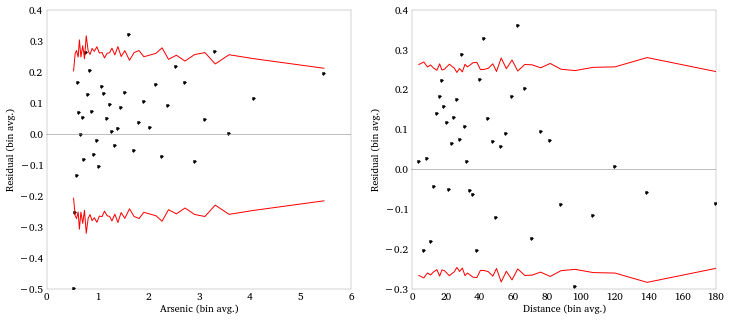
\includegraphics[width=0.7\textwidth]{stat_wells_files/stat_wells_fig_04.png}
\par
\end{center}
\end{codeoutput}
\end{codecell}
\subsubsection{Model hata oranlari}

\texttt{pred\_table()} cagrisi bize bu modelin ``kafa karisikligi
matrisini (confusion matrix)'' veriyor. Bu matrisi kullanarak
modelimizin hata oranini hesaplayabiliriz.

Sonra bu sonucu, en fazla verilen cevabi herkesin cevabiymis gibi
farzeden daha basit bir ``null modelinin'' hata orani ile
karsilastirmaliyiz. Mesela burada kisilerin \%58'i kuyu degistirmis, bu
durumda null modeli ``herkes kuyu degistiriyor'' diye modeller, ve bu
basit modelin hata payi 42\% olur. Bizim model bu modelden daha iyi bir
sonuc verecek midir? Sonuc altta.

\begin{codecell}
\begin{codeinput}
\begin{lstlisting}
print model5.pred_table()
print 'Model Error rate: {0: 3.0%}'.format(
    1 - np.diag(model5.pred_table()).sum() / model5.pred_table().sum())
print 'Null Error Rate: {0: 3.0%}'.format(
    1 - df['switch'].mean())
\end{lstlisting}
\end{codeinput}
\begin{codeoutput}
\begin{verbatim}
[[  568.   715.]
 [  387.  1350.]]
Model Error rate:  36%
Null Error Rate:  42%
\end{verbatim}
\end{codeoutput}
\end{codecell}
{[}1{]} https://patsy.readthedocs.org/en/v0.1.0/formulas.html

{[}2{]}
http://nbviewer.ipython.org/urls/raw.github.com/carljv/Will\_it\_Python/\\
master/ARM/ch5/arsenic\_wells\_switching.ipynb

{[}3{]} Eger bir katsayi degerinin sifirdan uzakligi Std. Hatanin
(Error) iki katindan fazla ise katsayi istatistiki olarak anlamli /
degerli (significant) demektir ve kullanilabilir. Tabii burada biraz
daha ek irdeleme gerekebilir; mesela kisilerin arabalarinin beygir
gucunu kazandiklari maasa baglayan bir regresyon, beygir gucu katsayisi
icin beygir basina \$10 ve std. hata \$2 vermisse bu istatistiki olarak
onemli, ama pratikte onemsizdir. Benzer sekilde eger beygir katsayisi
icin \$10,000 ve std. hata \$10,000 bulmussak, bu istatistiki olarak
onemsiz, ama pratikte onemlidir.

\end{document}
